\documentclass{beamer}
\usepackage[utf8]{inputenc} 
\usepackage[spanish]{babel} % Para soporte en español
\usepackage{minted} % Importar el paquete listings
\usetheme{Madrid} % Puedes elegir otro tema si lo prefieres


\title{Arquitectura de una Computadora}
\subtitle{Computadoras y programas}
\author{Irving Josue Flores Romero}
\date{\today}

\begin{document}
	
	\begin{frame}
		\titlepage
	\end{frame}
	
		\begin{frame}{Entscheidungsproblem}
		
		\begin{itemize}
			\item \textbf{David Hilbert propuso en 1990 el Entscheidungsproblem} : Existe un algoritmo general capaz de resolver si un enunciado matematico es verdadero o falso?
			\item \textbf{Solucón:} En 1963 Alonso Chuch y Alan Turing demostraron que no existe tal algoritmo.
			\item \textbf{Implicaciones:} Crearon las bases de las computadoras actuales.
		\end{itemize}
		
	\end{frame}
	
	\begin{frame}{La Máquina de Turing}
		
		\begin{itemize}
			\item \textbf{Definición formal:} 
			Una máquina de Turing es una 7-tupla $M = (Q, \Sigma, \Gamma, \delta, q_0, F, \sqcup)$, donde:
			
			\begin{itemize}
				\item $Q$ es un conjunto finito de \textit{estados}.
				\item $\Sigma$ es un conjunto finito de \textit{símbolos de entrada}.
				\item $\Gamma$ es un conjunto finito de \textit{símbolos de cinta}, que incluye $\Sigma$.
				\item $\delta : Q \times \Gamma \rightarrow Q \times \Gamma \times \{L, R\}$ es la \textit{función de transición}.
				\item $q_0 \in Q$ es el \textit{estado inicial}.
				\item $F \subset Q $ es el \textit{conjunto de estados finales}.
				\item $\sqcup$ es el \textit{simbolo blanco}, donde $\sqcup \in \Gamma$ pero  $\sqcup \notin \Sigma$.
			\end{itemize}
		\end{itemize}
		
	\end{frame}
	
	\begin{frame}{La Máquina de Turing}
		
			\begin{figure}
			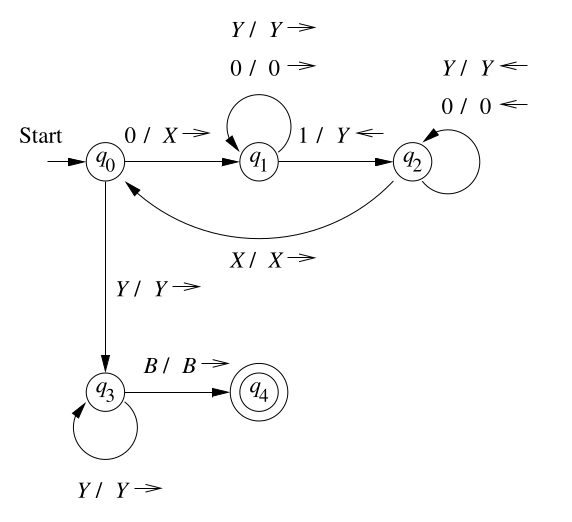
\includegraphics[width=0.5\textwidth]{diagrama_estados.png} 
			\caption{Diagrama de estados de una maquina de Turing}
			\end{figure}
		
	\end{frame}
	
		
	\begin{frame}{La Máquina universal de Turing}
		
		\begin{itemize}
			\item Es posible codificar una maquina de turing en una cadena de simbolos. (Estados, funcion de transición, etc.)
			\item Existe una maquina de Turing capaz de procesar como entrada otra maquina de Turing junto una palabra y producir el mismo resultado.
		\end{itemize}
		\begin{figure}
			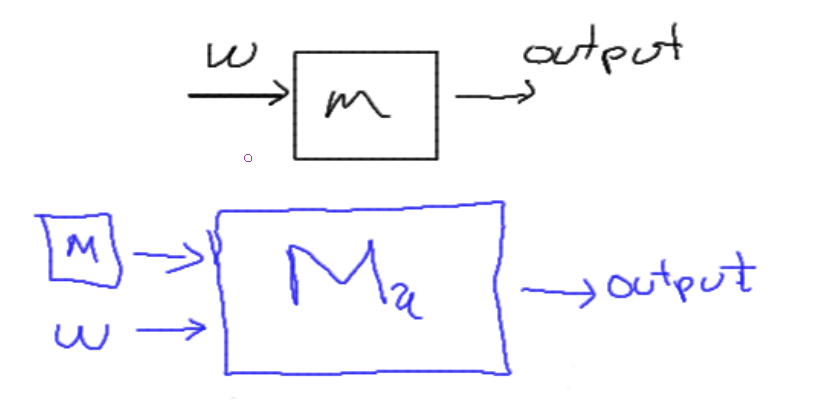
\includegraphics[width=0.5\textwidth]{maquina_universal.png}
		\end{figure}
		
	\end{frame}
	
	
	\begin{frame}{Problema de la parada}
		
		\begin{itemize}
			\item \textbf{Problema de la parada:} ¿Existe una maquina $M_p$ tal que dada una maquina $M$ y una palabra $w$ la maquina $M_p$ muestre como salida $p$ si la maquina $M$ termina en un numero finito de pasos o $n$ si no?.
			\pause
			\item \textbf{No existe!}
		\end{itemize}
		
		
	\end{frame}
	
		\begin{frame}{Conclusión}
		
		\begin{itemize}
			\item Existen problema indecidibles.
			\item Las maquinas de turing dan un indicio de como puede construirse una computadora física.
			\item Existe una maquina universal \textit{programable}.
		\end{itemize}
		
		
	\end{frame}
	
	
	
	\begin{frame}{¿Qué es un compilador?}
		
		\begin{itemize}
			\item Un compilador es un programa que traduce un programa escrito en un lenguaje de alto nivel (como C++, Java, Python) a un lenguaje de bajo nivel (como lenguaje ensamblador o código máquina).
			\item Esta traducción permite que el programa sea ejecutado por una computadora.
		\end{itemize}
		
	\end{frame}
	
	\begin{frame}{Compiladores, Intérpretes y Transpiladores}
		
		\begin{itemize}
			\item \textbf{Compilador:} Traduce todo el código fuente a código máquina antes de la ejecución. El programa resultante se ejecuta directamente en el hardware.
			\item \textbf{Intérprete:} Lee y ejecuta el código fuente línea por línea, sin generar un programa ejecutable independiente.
			\item \textbf{Transpilador:} Traduce código fuente de un lenguaje de alto nivel a otro lenguaje de alto nivel. El código resultante puede ser ejecutado por otro intérprete o compilador.
		\end{itemize}
		
	\end{frame}
	
	\begin{frame}{Etapas de la Compilación}
		
		\begin{figure}
			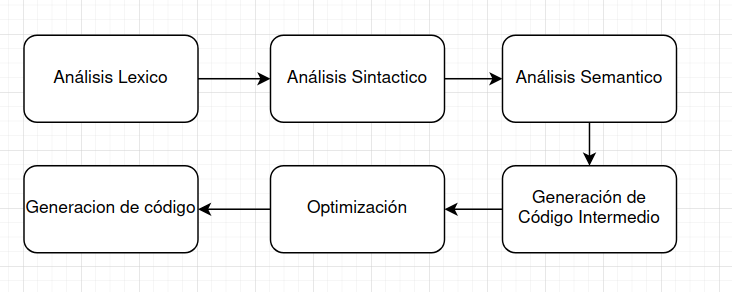
\includegraphics[width=0.8\textwidth]{diagrama_compilador.png} % Reemplaza con la ruta a tu imagen
			\caption{Esquema general de las etapas de un compilador}
		\end{figure}
		
	\end{frame}
	
	\begin{frame}[fragile]{Análisis Léxico}
		
		\begin{itemize}
			\item El analizador léxico (o scanner) lee el código fuente carácter por carácter y lo agrupa en tokens (palabras clave, identificadores, operadores, etc.).
			\item Ignora espacios en blanco y comentarios.
		\end{itemize}
		\vspace{1cm} % Espacio vertical de 1 centímetro
		\pause
			\begin{minted}[
				framesep=2mm,
				baselinestretch=1,
				fontsize=\scriptsize,
				obeytabs=true,tabsize=2
				]{c}
						int x;
						x = 5;
						// Lista de tokens
						// int, x, ;, x, =, 5, ;
			\end{minted}
	\end{frame}
	
	\begin{frame}[fragile]{Análisis Sintáctico}
		
		\begin{itemize}
			\item El analizador sintáctico (o parser) verifica que la secuencia de tokens siga las reglas gramaticales del lenguaje.
			\item Construye un árbol sintáctico que representa la estructura del programa.
		\end{itemize}
		\pause
		\begin{verbatim}
      Programa
							/   		\
Declaración   Asignación
			/      			    /   \
		int        		  x     5
		|
		x
		\end{verbatim}
	\end{frame}
	
	
	\begin{frame}[fragile]{Análisis Semántico}
		
		\begin{itemize}
			\item El analizador semántico verifica que el programa tenga sentido.
			\item Comprueba tipos de datos, declaraciones de variables, etc.
		\end{itemize}
		\pause
		\begin{minted}[
			framesep=2mm,
			baselinestretch=1,
			fontsize=\scriptsize,
			obeytabs=true,tabsize=2
			]{c}
			int x;
			x = "hola";
			y = 4.5;
		\end{minted}
	\end{frame}
	
	\begin{frame}{Generación de Código Intermedio}
		
		\begin{itemize}
			\item Se genera una representación intermedia del programa, independiente de la máquina de destino.
			\item Facilita la optimización y la portabilidad.
		\end{itemize}
		
	\end{frame}
	
	\begin{frame}{Optimización}
		
		\begin{itemize}
			\item Se mejora el código intermedio para que sea más eficiente (más rápido o que ocupe menos memoria).
		\end{itemize}
		
	\end{frame}
	
	\begin{frame}{Generación de Código}
		
		\begin{itemize}
			\item Se traduce el código intermedio al lenguaje de la máquina de destino.
		\end{itemize}
		
	\end{frame}
	
	\begin{frame}{Generadores Automáticos}
		
		\begin{itemize}
			\item Herramientas que facilitan la creación de analizadores léxicos y sintácticos.
			\item Ejemplos: Lex/Flex, Yacc/Bison, ANTLR.
			\item A partir de una especificación formal de la gramática del lenguaje, generan el código del analizador.
		\end{itemize}
		
	\end{frame}
	
		\begin{frame}{Ejercicio}
		Cree un compilador que reconozca lo siguiente
		\begin{itemize}
			\item Debe recibir el comando \texttt{saludo} seguido de los nombres que se necesitan saludar separados por espacio.
			\item Los nombres pueden ser un string cualquiera o un hashtag seguido de uno de los siguientes sujetos \texttt{\#cantante}, \texttt{\#actor}, \texttt{\#prota}.
			\item La salida del programa debe ser un programa en \textit{c} o \textit{python} que ejecute los saludos.
		\end{itemize}
		
	\end{frame}
	
		\begin{frame}[fragile]{Ejercicio}
			Entrada al compilador
		\begin{minted}[
			frame=lines,
	framesep=2mm,
	baselinestretch=1,
	fontsize=\scriptsize,
	obeytabs=true,tabsize=2
	]{vim}
	saludo irving @pi_314 #prota
\end{minted}
Salida al compilador
		\begin{minted}[
	frame=lines,
	framesep=2mm,
	baselinestretch=1,
	fontsize=\scriptsize,
	obeytabs=true,tabsize=2
	]{vim}
	print("Hola irving")
	print("Hola @pi_314")
	print("Hola Eren Jaeger")
\end{minted}
		
	\end{frame}
	
\end{document}